\documentclass[11pt,a4paper,english]{scrreprt}
\usepackage[utf8]{inputenc}
\usepackage[T1]{fontenc}
\usepackage{lmodern}

\usepackage[english]{babel}
\usepackage{csquotes}
\usepackage[long,nodayofweek,level,24hr]{datetime} 
\usepackage[skip=5pt,font=footnotesize]{caption}

\usepackage{tabularx}
\usepackage{booktabs}
\usepackage{amsmath}
\usepackage{amssymb}
\usepackage{graphicx}
\usepackage{subfigure}
\usepackage{enumitem}
\usepackage[table]{xcolor}
\usepackage{xcolor}
\usepackage[bookmarksnumbered]{hyperref}
\hypersetup{pdfborder={0 0 0}, breaklinks=true}
\usepackage{bookmark}
% \addtokomafont{disposition}{\rmfamily}
\usepackage[onehalfspacing]{setspace}

% DISABLE TODO NOTES HERE %%%%%%%%%%%%%%%%%%%%%%%%%%%%%%%%%
\usepackage{todonotes}
%\usepackage[disable]{todonotes}

% HEADER & FOOTER DEFINITIONS %%%%%%%%%%%%%%%%%%%%%%%%%%%%%
\usepackage{fancyhdr}
\pagestyle{fancy}
\renewcommand{\headrulewidth}{0pt}
\fancyhead{}
\fancyfoot{}
\fancyfoot[R]{\textcolor{gray}{\thepage}}

\fancypagestyle{plain}{%
    \renewcommand{\headrulewidth}{0pt}%
    \fancyhf{}%
    \fancyfoot[R]{\textcolor{gray}{\thepage}}%
}

% LITERATURE %%%%%%%%%%%%%%%%%%%%%%%%%%%%%%%%%%%%%%%%%%%%%
\usepackage[backend=biber,style=apa]{biblatex}
\addbibresource{literatur.bib}


% DEF FOR COVER %%%%%%%%%%%%%%%%%%%%%%%%%%%%%%%%%%%%%%%%%%
\newcommand{\titelMAEnglish}{Explainable Artificial Intelligence:\\ Designing human-centric assessment system interfaces to increase explainability and trustworthiness of artificial intelligence in medical applications}

\newcommand{\authorMA}{Philipp Dominik Bzdok}

\newcommand{\examinerMA}{Univ.-Prof. Dr. rer. nat. Thomas Franke, Dipl.-Psych.}

\newcommand{\supporterMA}{Tim Schrills, M.Sc.}
%%%%%%%%%%%%%%%%%%%%%%%%%%%%%%%%%%%%%%%%%%%%%%%%%%%%%%%%%%%

% DEF FOR COMMENTS, CAN BE DELETED %%%%%%%%%%%%%%%%%%%%%%%%
\newenvironment{comment}
  {\par\medskip
   \begingroup\color{olive}%
   }
 {\endgroup
  \medskip}
%%%%%%%%%%%%%%%%%%%%%%%%%%%%%%%%%%%%%%%%%%%%%%%%%%%%%%%%%%

\begin{document}
\pagenumbering{gobble}
\begin{titlepage}
    \begin{figure}[t]
        \centering
        
\includegraphics[width=0.7\textwidth]{img/UzL_Logo.png}
    \end{figure}
    \todo{English Logo}
    \begin{center}
        \fontfamily{phv}\selectfont
        \textcolor{gray}{Director: Prof Dr. rer. nat. Michael Herczeg}\\
        \vspace*{1.5cm}
        \Large
        \begin{onehalfspace}
            \textbf{\titelMAEnglish}
        \end{onehalfspace}
        \vspace{1cm}
        \normalsize
        \textbf{Master's Thesis}\\
        \vspace{0.2cm}
        as part of the study program\\
        \textbf{Media Informatics}\\
        of the University of Lübeck\\
        \vspace{1cm}
        submitted by:\\ \textbf{\authorMA}\\
        \vspace{1cm}
        Issued and supervised by:\\ \textbf{\examinerMA}\\
        \vspace{0.5cm}
        with support from:\\ \textbf{\supporterMA}\\
        \vspace{1cm}
        Lübeck, \today
    \end{center}        
\end{titlepage}
\setlength{\parindent}{0em}
\setlength{\parskip}{1em}

\begin{comment}
\begin{center}
    \textbf{Vorbemerkung}

    (Version: 2021-05-12-IMIS LaTex Version by Philipp Bzdok)
\end{center}
Anbei ein kommentiertes Template für Projekt- und Abschlussarbeiten in der Medieninformatik. Die grünen Kommentare in jedem Fall vor einer (Zwischen-) Abgabe entfernen (alle!).

Alle Angaben sind eigene Einschätzung (bzw. aus den zitierten Quellen, die aber auch wieder nach eigenen Überlegungen von mir ausgewählt wurden) und entsprechend ohne Gewähr. Nordstrom's Policy gilt auch hier: "Use your own best judgment at all times.".

Es ist ihre Arbeit. Sie investieren 6 Monate Ihrer Lebenszeit in die Arbeit und Sie müssen Sie vor anderen verteidigen. Sehen Sie Hinweise von anderen als Ratschläge: Ernst nehmen, aber immer für sich selbst entscheiden, was passt, was nicht und was auf ein Problem hinweist, was man dann aber anders löst.
Das letzte Wort (v.a. über formelle Aspekte) hat allerdings immer der jeweilige Betreuer.

Zunächst kommen ein paar allgemeine Vorbemerkungen, die für die ganze Arbeit relevant sind (Allgemeine Punkte der Arbeit). Danach die Gliederung einer normalen Arbeit mit Anmerkungen in den entsprechenden Kapiteln bzw. Abschnitten.

Viel Erfolg beim Schreiben.

Daniel Wessel

\textbf{Rundumschlag was wissenschaftliches Arbeiten betrifft:}\\ \url{https://www.youtube.com/watch?v=_ID7q7pXzyc}

\textbf{Allgemeine Punkte der Arbeit}
\begin{itemize}
    \item \textbf{Änderbarkeit von Struktur und Inhalten:} Je nach konkretem Thema kann eine andere Struktur sinnvoll sein. Dies ist ins-besondere bei der Reihenfolge der Analyse-Abschnitte der Fall, kann aber auch ganze Kapitel betreffen. Das ist insbesondere bei Masterarbeiten der Fall, die sich je nach Ausrichtung (z. B. theoretische Arbeit) stark von der sonst üblichen Form unterscheiden. Diese Struktur so früh wie möglich mit dem Betreuer klären, ihm dann per eMail zuschicken und sich kurz bestätigen lassen (generell hat man viel zu tun und erinnert sich nicht unbedingt an alle Absprachen, deswegen einfach im Anschluss kurz eine Zusammenfassung des Gesprächs per eMail schicken).
    \item \textbf{Exposé (Bachelor-/Masterarbeit) bzw. Pflichtenheft (Bachelor-/Masterprojekt) setzt die inhaltliche Bewertungsgrundlage:}  Darin haben Sie (Arbeit) oder Ihr Betreuer (Projekt) festgelegt, was zu erreichen ist. Entsprechend genau überlegen, was man verspricht bzw. zu was man sich verpflichtet.
    \item \textbf{Zielgruppe:} Schreiben Sie die Arbeit so, dass andere Personen verstehen, was Sie machen — auch wenn sie keine (Medien-)Informatik studiert haben. Sprich: Beginnen Sie breit um den Einstieg zu erleichtern und formulieren Sie es allgemein verständlich (z. B. das die öffentliche Verwaltung zunehmend digitalisiert wird) und fassen Sie am Ende eines Kapitels die Punkte allgemeinverständlich wieder zusammen. Dazwischen können Sie auf ein Detaillevel runtergehen und eine Komplexität nutzen, die ein Laie nicht mehr versteht. Da der Text in Absätzen aufgebaut ist, kann der Laie (oder nicht interessierte) diese Absätze überspringen. Der Laie sollte aber zumindest im Prinzip verstehen, was Sie gemacht haben.
    \item \textbf{Roter Faden:} Die Arbeit logisch aufeinander aufbauen: In der Einleitung legen Sie dar, was Sie erreichen wollen und zeigen dabei auch subtil, warum das wichtig / interessant / relevant ist (\textit{"Why should I care?"}). Das geschieht über Belege und Argumente, wann immer Sie "wichtig", "interessant" oder "relevant" im Text verwenden sind Sie dabei gescheitert. \textbf{Alle} Kapitel nach der Einleitung zeigen \textbf{logisch aufeinander folgend}, wie der Zweck der Arbeit erreicht wird.
    \item \textbf{Zwischenstufen-Denken:} So schreiben, dass am Ende jedes Kapitels (Einleitung, Analyse, Konzeption, Realisierung, Dialogbeispiele, Evaluation) der Leser stoppen könnte und die Arbeit selbst fortführen könnte (z. B. nach der Einleitung sich für eine anderes Analysevorgehen entscheiden, oder auf Basis der Analyse eine andere Lösung konzipieren).
    \item \textbf{Eigenes Fazit am Ende jeden Kapitels — Was bedeuten die Ergebnisse für die Arbeit bzw. deren Ziel?} Z. B. am Ende der Analyse kurz zusammenfassen, was die wesentlichen Punkte für die weitere Entwicklung sind — mit Fokus auf das nächste Kapitel (hier: Konzeption). Am Ende der Konzeption kurz zusammenfassen, was die wesentlichen Punkte für die weitere Entwicklung (jetzt: Realisierung) sind, etc. pp. Ein gutes Fazit ist viel Arbeit und setzt ein gut geschriebenes Kapitel voraus.
    \item \textbf{Professionelle Zwischenabgaben:} Wenn Sie den Text an den Betreuer geben, gehen Sie vorher kritisch drüber. Wenn Textmarken falsch gesetzt sind, die Formatierung zusammengebrochen ist, etc. dann muss sich der Betreuer da erst mal durchwühlen um zum Inhalt zu kommen. Gute Formatierung macht keine schlechte Arbeit gut (die inhaltlichen Fehler fallen eher umso deutlicher auf), aber schlechte Formatierung macht eine gute Arbeit schlechter.
    \item \textbf{Professionell und offen Kommunizieren:} Weder sich selbst kreuzigen noch Fehler verbergen, sondern berichten, was gemacht wurde und mit Fehlern konstruktiv umgehen.
\end{itemize}

\textbf{Sprache: Stil}
\begin{itemize}
    \item \textbf{Kein Ich, keine Hero's Journey:} Es ist — im Prinzip — egal, wer die Arbeit durchgeführt hat (zumindest für die Qualität der Arbeit, nicht für die Bewertung Ihrer Leistung). Was überzeugen muss ist das Vorgehen, die Belege und Argumentation. Entsprechend stellen Sie das Vorgehen neutral dar ohne auf sich selbst zu verweisen (eher passiv verwenden). Ausnahmen sind u.a. in Danksagung, Widmung, Eidesstattliche Erklärung.
    \item \textbf{Meta vermeiden}: Sie müssen an vielen Stellen darauf hinweisen was kommt (z. B. zu Beginn eines jeden Kapitels). Reißen Sie den Leser aber dabei nicht aus dem Text. Mental ist der Leser dabei, ihre Arbeit zu beobachten, was Sie konkret getan haben. Wenn Sie ihm jetzt sagen "In diesem Kapitel ..." dann ziehen Sie ihn aus dem Text und bringen ihn dazu, über den Text nachzudenken statt über das, was gemacht wurde. Bleiben Sie bei dem, was Sie gemacht haben, z. B. "Nachfolgend werden ...". 
    \item \textbf{Kapitel $\neq$ Unterkapitel $\neq$ Abschnitt:} 1 ist ein Kapitel, 1.1 ein Unterkapitel, 1.1.1 ein Abschnitt, 1.1.1.1 existiert nicht. Wenn Sie noch mehr Einteilungen brauchen, dann verwenden Sie Abschnitte mit Fettdruck zu Beginn (wie in diesem Abschnitt, dann aber ohne die Bulletpoints).
    \item \textbf{Kein Bulletpoint-Text:} Bulletpoints sind nur an wenigen Stellen hilfreich, z. B. bei Aufzählungen. Sätze nie mit Bulletpoints aufzählen. Entweder die Sätze auf Stichworte reduzieren oder eine Tabelle draus machen.
    \item \textbf{Auch digital gedrucktes ist tot und macht nichts mehr:} Sie berichten was Sie gemacht haben — außerhalb des Berichtes. Entsprechend nie schreiben, dass z. B. in der Analyse der Sachverhalt analysiert wird. Der Bericht macht von sich aus nichts. Sie stellen dort die Ergebnisse der Analyse dar.

    \item \textbf{Umgangssprache vermeiden, Hochgestochene Sprache vermeiden:} Weder Umgangssprache (Sozialpädagogensprache; "tut", "Das Ganze ...", "etwas für ihre Gesundheit zu machen") noch Hochgestochen (à la Philosophendeutsch) schreiben. Wissenschaftliche Sprache ist nach \textcite{alley_1996}:
    \begin{itemize}
        \item präzise: sagen was man meint (richtige Wort, richtiges Detaillevel)
        \item klar: vermeiden Sachen zu sagen/implizieren, die man nicht meint, d.h. Ambiguität und unnötige Komplexität (v.a. in der Wahl der Wörter) vermeiden
        \item ehrlich: direkt und offen kommunizieren
        \item prägnant: jedes Wort sollte zählen
        \item bekannt/vertraut: neue Fakten in bekannten Kontext verankern
        \item flüssig: von Satz zu Satz, Absatz zu Absatz, ohne dass der Leser stolpert
    \end{itemize}
    \fullcite{alley_1996}
\end{itemize}

\textbf{Sprache: Zeitformen}
\begin{itemize}
    \item \textbf{In einem Bericht berichten Sie:} Entsprechend Vergangenheitsform verwenden. Sie berichten über eine abgeschlossene Arbeit, selbst wenn diese noch läuft als Sie es geschrieben haben, und selbst bei Zielen der Arbeit. Ausnahmen sind selten, z. B. bei den Ergebnissen ("Daten zeigen ..." — sie machen es ja noch) und Aus-blick bzw. Vorschläge für die Zukunft.
\end{itemize}

\textbf{Sprache: Absätze}
\begin{itemize}
    \item \textbf{Eine Sinneinheit = 1 Absatz:} Absätze behandeln immer einen Punkt, eine Sinneinheit. Wenn eine halbe Seite lang kein Absatz verwendet wird, liegt meist ein Problem vor.
    \item \textbf{Absätze sind immer länger als ein Satz:} Keine Einsatz-Stückel-Absätze. Einzige Ausnahme: Sie wollen, dass der Leser die komplette Aufmerksamkeit auf diesen zentralen Satz lenkt. Das kann man 1-2 Mal in einer Arbeit machen.
\end{itemize}

\textbf{Interne Verweise}
\begin{itemize}
    \item \textbf{Verweise statt Wiederholungen:} Üblicherweise braucht man einen Sachverhalt nur ein Mal zu beschrieben — dann verweist man an anderer Stelle auf den konkreten Abschnitt. Das ist auch der Grund für die Nummerierung — es erlaubt Ihnen, den Leser präzise zu den Punkt in der Arbeit zu schicken, an dem Sie auf den Sachverhalt eingehen. Nutzen Sie also "wie in der Kontextanalyse (2.4) beschrieben ...", dann weiß der Leser, wie lange er blättern muss.
\end{itemize}

\textbf{Zitationen}
\begin{itemize}
    \item \textbf{APA verwenden:} American Psychological Association (7. Ausgabe) Stil verwenden. Gibt genug Informationsseiten dazu im Netz und Literaturmanager können diesen Stil üblicherweise.
    \item \textbf{Richtige Zitationen:} Falsche "ich füg die richtigen Zitationen später ein" Ab-gaben verbrennen Ihnen den Betreuer. Arbeiten Sie von Anfang an mit einem Literaturverwaltungsprogramm, in dem die verwendeten Quellen richtig eingetragen sind (nächster Punkt).
    \item \textbf{Autorennamen müssen genannt werden, aber nicht hervorheben:} Die Wissenschaft sollte keinen Personenkult kennen — das können gerne Religionen oder Ideologien übernehmen. Wer was herausgefunden hat, ist egal. Die Qualität der Arbeit zählt. Entsprechend nicht "Die Autoren xyz haben herausgefunden das ABC vor-liegt" sondern "Da ABC vorliegt (Autoren Jahr) ...".
    \item \textbf{Kein Paper-Denglish:} Ja, im englischen heißt es Paper. Im Text sind es aber Artikel oder Konferenzbeiträge oder Buchkapitel oder was auch immer. Üblicherweise muss man den Typ auch nicht erwähnen (im Normalfall wurde man eh Artikel/Konferenzbeiträge zitieren). Bitte nicht so was wie "Im Paper von xyz ...", das klingt nach Möchtegern-coole Manta mit Fuchsschwanz Sprechweise. Ein-fach berichten wie die Befundlage ist, über Autorenname und Jahr (meist in Klammern) belegen wo es herkommt (sonst ein Plagiat) und die Belege und Argument in der Arbeit sprechen lassen.
    \item \textbf{Wörtliche Zitate nur wenn es nicht anders geht:} In den meisten Fällen geben Sie Befunde oder Argumente mit Ihren eigenen wieder (mit Quellenangabe). Wörtliche Zitate braucht man nur in sehr seltenen Fällen. Z. B. treffende Aussage von Evaluationsteilnehmern, oder eine Definition, die man 1:1 so sagen muss.
    \item \textbf{Fußnoten vermeiden:} Entweder es ist wichtig genug, genannt zu werden, oder es ist so unwichtig, dass es raus kann. Fußnoten reißen den Leser aus dem Text. Einzige Ausnahme: Bei der ersten Verwendung des generische Maskulinums.
    \item \textbf{Es gibt mehr Plagiate als nur Quellen nicht angeben:} Es gibt z. B. Übersetzungsplagiate, bei denen Sie einen Text(teil) einfach auf deutsch übersetzen ohne die Quelle anzugeben, oder dass man einfach die Argumentstruktur und Quellenangaben aus einem anderen Text übernimmt (ohne die Quelle anzugeben). Sie schmücken sich dann mit fremden Federn und Blender sind selten willkommen.
    \item \textbf{Literaturverwaltungsprogram nutzen:} Literaturverwaltungsprogramm (z. B. Zotero) hilft extrem bei der richtigen Zitierung, aber ACHTUNG: Wenn die Angabe in Zotero fehlt, ist auch die automatische Generierung des APA Stils falsch! GIGO gilt auch hier.
\end{itemize}

\textbf{Abbildungen und Tabellen}
\begin{itemize}
    \item Expliziter Verweis vom Text auf die Abbildung/Tabelle immer im Absatz vor der Abbildung/Tabelle (Leser stolpern über Abbildung/Tabelle, suchen dann nach oben nach mehr Informationen).
    \item Auf \textbf{Lesbarkeit} achten! Schriftgröße und Auflösung (bei Bildern) im Probedruck überprüfen!
    \item Für Schwarz/Weiß-Druck und für Farbfehlsichtige geeignet.
    \item Tabellen nach \textbf{APA Stil} (nur horizontale Linien und nur nach Header oder vor Footer.
\end{itemize}

\textbf{Druck}
\begin{itemize}
    \item Arbeit einseitig drucken!
    \item \textbf{PDF Druck und Suchfunktion:} Zuerst als PDF drucken, dann nach "Fehler! Verweisquelle konnte nicht gefunden werden." suchen. Word bricht schon mal gerne die Verlinkungen und das sieht man erst im Druck! Generell PDF Dokument kritisch durchgehen und PDF auch zum Drucken im Copyshop verwenden!
    \item Nach dem Druck und vor dem Binden alle Seiten selbst sowie von einer anderen Person durchgehen (lassen).
\end{itemize}
\end{comment}
\newpage
\chapter*{Danksagung}
\begin{comment}
Kurzer Dank an Personen, die Sie bei der Arbeit unterstützt haben. Z. B. inoffizielle Betreuer, Teilnehmer an den Evaluationen (nie namentlich nennen), Medientechnik, Sekretärin, etc. pp. — nur wenn Sie den Personen wirklich dankbar sind. (Ist nett aber für die Bewertung irrelevant.)
Falls nicht verwendet diese Seite einfach entfernen.
\end{comment}

Text \dots

\newpage
\chapter*{Kurzfassung}
\begin{comment}
Abstract schon für Zwischenabgabe schreiben. Später kommen dann noch Sätze dazu, aber Grundgerüst steht.

Kein "Teaser" sondern eine kurze Zusammenfassung (das, was man braucht, um sich schnell einen Überblick zu verschaffen, ob es sich lohnt, die Arbeit zu lesen).

Inhalt umfasst die zentralen Punkte aller Kapitel, von Ziel/Fragestellung bis Ausblick.

Nie länger als diese eine Seite (inkl. Schlüsselwörter).
\end{comment}

Text \dots

\section*{Schlüsselwörter}
\begin{comment}
Verwendete Literatur gibt Hinweise auf passende Stichwörter. Das sind die Suchbegriffe, die man bei einer Literatursuche verwenden würde.
\end{comment}

Text \dots

\newpage
\chapter*{Abstract}
\begin{comment}
Englische Version der Kurzfassung.
Nicht einfach Google Translate oder DeepL verwenden. Trifft die Nuancen nicht und klingt z. T. nach Yoda.
\end{comment}

Text \dots

\section*{Keywords}
Text \dots

\newpage
\tableofcontents

\newpage
\pagenumbering{arabic}
\chapter{Introduction}
The use of Artificial Intelligence (\textbf{AI}) has risen rapidly in many application fields such as image processing, multimedia and gaming \parencite{jordan_machine_2015}. Other application domains, such
as medical systems, cannot benefit as easily from AI-based technological innovation compared to
recreational domains. This impediment oftentimes stems from the AI being a "black box". In consequence humans struggle to understand such systems and their decisions leading to trust and
compliance issues \parencite{adadi_blackbox_2018}. These issues are further enhanced in the medical
context where decisions, possibly based on AI, can have catastrophic consequences for users,
especially patients.

An example for medical human-AI interaction is the image-guided recognition of Deep Vein Thrombosis (\textbf{DVT}) with real-time AI support for medical professionals by \textit{ThinkSono} \parencite{thinksono_website}. Closely related in this context is the currently ongoing interdisciplinary research project \textit{CoCoAI}, which aims to explore psychological, ethical and technological implications of human-centered, AI-based applications in the DVT diagnosis and beyond \parencite{cocoai_website}. \textcite{ribeiro_why_2016} already explored the importance of explainability and trust in AI-based systems and proposed algorithms for model-agnostic explanations. Furthermore recent technological advances are realized by \textit{Clearbox AI}, with the focus on trustworthy AI by implementing an AI model assessment \parencite{clearbox_website, eu_trustworthy_ai}. The model assessment can help model owners to identify robustness issues, potential undesired behaviour, and explain errors and uncertainties regarding the model predictions \parencite{clearbox_wp}.

Explainable Artificial Intelligence (\textbf{XAI}) plays an important role in the acceptance and finally in the usage of AI-based technology. This is further underlined in the medical context where public authorities set strict regulations on the usage of technological systems. XAI is a research field that studies how AI decisions and data driving those decisions can be explained to people in order to provide transparency, enable assessment of accountability, demonstrate fairness, or facilitate understanding \parencite{arrieta_explainable_2019}.

Trust in AI systems is primarily induced by the users' understanding and the general interpretability of the machine learning model and their predictions \parencite{ribeiro_why_2016, ras_explanation_2018}. The wide array of different possible user groups and the complex constructs of understandability and trust demands for a human-centric approach in designing AI assessment systems. Because of the inherent complexity of non-linear machine learning models, especially Deep Neural Networks (\textbf{DNNs}) for real-time image processing, suitable visualization and communication techniques are non-trivial and a primary focus of this work. Additionally to the complex models for image classification, the input data is also more complex as it is unstructured. Non-linear neural networks and unstructured data provide additional challenges for XAI, as described in \textcite{keane_how_2019}. Furthermore \textcite{samek_explaining_2021} give an overview on the technical foundations of XAI and a presentation of practical algorithms, which will be used in conjunction with human-centric design to explore and evaluate suitable and efficient methods to explain a model classification with unstructured data by studying different alternatives ranging from perturbation based approaches to more model intrusive alternatives. 

In the context of a medical, image-based DVT diagnosis system, it is important that the responsible stakeholders, such as medical practitioners, specialized doctors and clinic managements, are enabled to make informed decisions on the usage of AI-based technology, even though their expertise in machine learning and data science is expected to be low. The stakeholders' trust in this system is a primary factor for the widespread adoption of said technology for real life applications. Therefore, increasing the understanding of the AI model and finding an optimal trust level in the predictions by designing human-centric explanation techniques within the AI model assessment system is a main goal of this work. Additionally it is conceivable that authorities will instantiate auditors for AI-based systems in medical contexts. Having a comprehensible and scientifically proven assessment system could be a big step in the approval and adoption of said system. 

\section{Goals}
\begin{comment}
\textbf{Konkretisieren:}Sie haben vor diesem Abschnitt gezeigt, worum es geht und warum es wichtig ist. Jetzt gehen Sie konkret auf die Ziele Ihrer Arbeit ein. Worum kümmern Sie sich und warum konkret das? Was haben Sie erreicht (Vergangenheitsform)?

\textbf{In einer Masterarbeit:} Die Forschungsfragen hier aufführen (eingerückt, leicht auf-findbar wenn man durchblättert). Die Fragen müssen sich logisch aus der Einleitung und den Zielen der Arbeit ergeben.
\end{comment}

Text \dots

\section{State of the Art}
\begin{comment}
\textbf{Nur falls Sie auf einem bestehenden System aufbauen:} Falls Sie ein System bekommen haben, das Sie weiter entwickeln, dann stellen Sie hier da, was das System kann (verständlich formulieren), wie es aussieht / aufgebaut ist (Screenshots!) und ggfs. wie es umgesetzt wurde (z. B. Klassendiagramm).

\textbf{Sobald Sie selbst nach Systemen suchen — sprich: eigene Recherchearbeit verwenden} — berichten Sie darüber besser in der Analyse. Schließlich beinhaltet eine Recherche auch immer eine Auswahl, und andere Personen hätten nach der Einleitung und den Zielen der Arbeit vielleicht anders gesucht (\textbf{vgl. Zwischenstufen-Denken}).
\end{comment}

Text \dots

\section{Approach}
\begin{comment}
\textbf{Einleitung als erste Schritt im menschzentrierten Gestaltungsprozess:} Die Vorgehensweise spiegelt im Prinzip das \textbf{Planen des menschzentrierten Gestaltungsprozesses wieder}. Das haben Sie im Exposé angefangen und hier (was dann tatsächlich gemacht wurde) überarbeitet dargestellt.

\textbf{Vorgehen:} Wie sind Sie vorgegangen, um die Ziele der Arbeit zu erreichen? Oft (aber nicht immer!) bietet sich das Diagramm aus der DIN EN ISO 9241-210 an (wenn Sie hier eine Abbildung verwenden, dann müssen Sie sich auch an das Vorgehen gehalten haben!).

\textbf{Orientierung im Bericht:} Wo findet der Leser die Ergebnisse der einzelnen Schritte und was beinhalten diese (kurz halten!)? Verweise auf Folgekapitel am besten im Stil "werden in der Analyse (Kapitel 2) ..." statt "in Kapitel 2 wird ..." — das Vorgehen gibt die Kapitel vor, nicht umgekehrt.
\end{comment}

\begin{figure}[htbp]
    \centering
    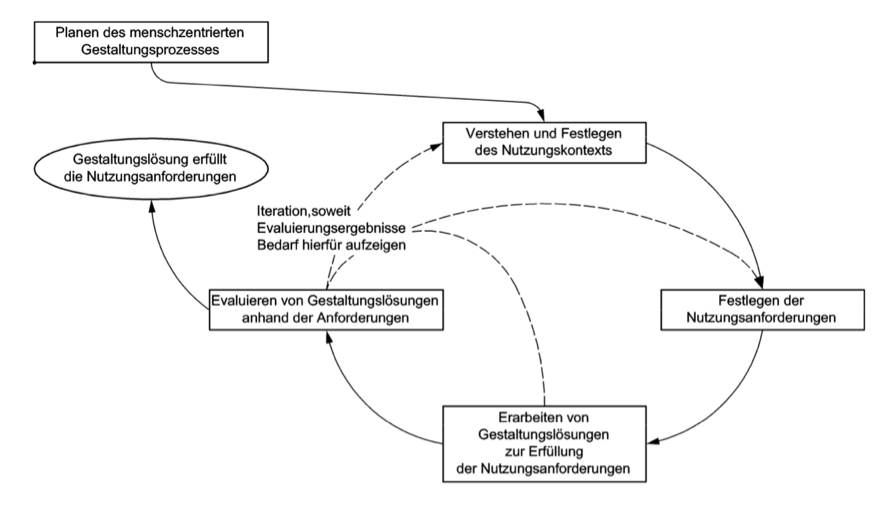
\includegraphics[width=\textwidth]{img/Picture1.png}
    \caption{Menschzentrierter Gestaltungsprozess \parencite{DIN}}
    \label{fig:picture1}
\end{figure}

Text \dots

\section{Definition of Terms}
Text \dots

\clearpage
\begin{comment}
\begin{center}
\huge
STOP\\
\normalsize
Halten Sie an dieser Stelle für einen Moment inne. Sie wissen, was Sie erreichen wollen, haben aber die Analyse noch nicht begonnen oder noch nicht abgeschlossen. Halten Sie auf einem Blatt Papier fest, wie Sie sich die Lösung für das Problem vorstellen. Wenn Sie mehrere Lösungen haben, um so besser. Legen Sie das Papier dann beiseite. Schauen Sie es auch erst einmal nicht mehr an.

Sie brauchen es erst \textbf{nach der ersten Iteration der Konzeption} wieder.
\end{center}
\end{comment}

\newpage
\chapter{Analysis}
\begin{comment}
\textbf{Über das Verstehen und Festlegen des Nutzungskontexts zum Festlegen der Nutzungsanforderungen:} Das Ziel der Analyse besteht aus den ersten beiden Iterationsschritte des menschzentrierten Gestaltungsprozesses: das \textbf{Verstehen und Festlegen des Nutzungskontexts}, was am Ende der Analyse im \textbf{Festlegen der Nutzungsanforderungen} mündet.

\textbf{Anforderungen verstehen, nicht schon Lösungen entwickeln:} Wenn Sie während der Analyse gute Ideen haben, dann diese sofort notieren. Aber in die Analyse kommt nur das, was für das Verstehen und Festlegen der Nutzungskontextes bzw. der Festlegung der Nutzungsanforderungen relevant ist. Ihre Ideen für Lösungen gehören in die Konzeption. Schließlich ist Ihre Lösung vermutlich nur eine von vielen und jemand, der nur bis zum Ende der Analyse liest, um dann selbst Lösungen zu konzipieren, sollte nicht von Ihren Lösungsideen beeinflusst werden.

\textbf{Advance Organizer:} An dieser Stelle (nach 2, vor 2.1) erfolgt eine kurze Übersicht, was den Leser in den Unterabschnitten erwartet. Das gibt dem Leser einen Überblick, wie Sie in Ihrer Analyse vorgegangen sind und erlaubt ihm zu interessanten Abschnitten zu springen. Gilt auch für alle weiteren Kapitel.

\textbf{Struktur der Analyse: }Die Reihenfolge der Analyse-Unterkapitel (Problemanalyse, Aufgabenanalyse, Benutzeranalyse, Kontextanalyse, Organisationsanalyse) muss eine logische Reihenfolge ergeben. Häufige Reihenfolgen (nach — falls sinnvoll — 2.1 Datenquellen) sind:

\begin{itemize}
    \item \textbf{Problem-/Aufgabenanalyse => Benutzeranalyse => Kontextanalyse => Organisationsanalyse:} "das ist das Problem/Aufgaben, das die Benutzer haben, die es unter den räumlichen und zeitlichen Bedingungen unter den organisationalen Rahmenbedingungen lösen müssen".
    \item \textbf{Benutzeranalyse => Problem-/Aufgabenanalyse => Kontextanalyse => Organisationsanalyse:} "die Benutzer sind gekennzeichnet durch (z. B. Patienten mit Depression), die aufgrund ihrer Eigenschaften die folgenden Probleme/Aufgaben haben, die sie unter den räumlichen und zeitlichen Bedingungen unter den organisationalen Rahmenbedingungen lösen müssen".
    \item \textbf{Organisationsanalyse => Problem-/Aufgabenanalyse => Benutzeranalyse => Kontextanalyse:} Organisationale Rahmenbedingungen haben sich verändert (z. B. zunehmende Digitalisierung), das führt zu neuen Problemen/Aufgaben bei den Benutzern, die es unter den räumlichen und zeitlichen Kontextbedingungen lösen müssen.
\end{itemize}

Wenn Sie die richtige argumentative Reihenfolge haben, können Sie die Analyse (sehr) abstrakt in einem Satz zusammenfassen (z. B. \textbf{Benutzeranalyse => Aufgabenanalyse => Problemanalyse => Kontextanalyse => Organisationsanalyse:} "Depressionspatienten sind durch verzerrte Erinnerungen gekennzeichnet, um die Therapie zu unter-stützen, müssen sie Ihre Emotionen protokollieren wenn diese auftreten, das ist allerdings ziemlich aufwändig und eine Lösung dafür muss nicht nur gebrauchstauglich sein, sondern auch unterwegs funktionieren und sich der Kommunikation mit dem Therapeuten und seiner Infrastruktur anpassen."). In den Unterkapiteln tragen Sie dann konkret zusammen, was für die menschzentrierte Gestaltung bezüglich Benutzer, Aufgabe, Problem, Kontext, und Organisation zu berücksichtigen ist. Sie tragen damit die Legobausteine für ihre Konzeption zusammen.

Häufig wird die Analyse allerdings dadurch erschwert, dass Sie unterschiedliche Probleme/Aufgaben haben, die von unterschiedlichen Benutzer(klassen) unter unterschiedlichen räumlichen und zeitlichen Bedingungen unter unterschiedlichen organisationalen Bedingungen ausgeführt werden (vgl. im Gegensatz zu der sehr speziellen eindeutige App für Depressionspatienten im klinischen Kontext z. B. ein allgemeines Programm wie Microsoft Word, das von einer sehr heterogenen Nutzergruppen verwendet wird).
\end{comment}

\section{Data Sources}
\begin{comment}
In Ihre Analyse verwenden Sie wahrscheinlich die selben Datenquellen (z. B. wissenschaftliche Literatur, bestehende Apps, Experteninterviews, Nutzerbefragungen, etc.) in mehreren Unterkapiteln. Hier können Sie diese Quellen kurz beschreiben um sie in den folgenden Unterkapiteln verwenden zu können. Das macht nur dann Sinn, wenn Sie die Daten auch wirklich in mehreren Unterkapiteln verwenden. Wenn Sie z. B. bestehende Apps nur in der Problemanalyse verwendet haben, dann das Vorgehen auch nur dort beschreiben (wäre allerdings was merkwürdig, wenn Ihnen die Apps nicht auch was über die anvisierten Nutzer sagen würde).

Generell müssen Sie die Quellen so beschreiben, dass jemand anders — wenn er das Vorgehen wiederholen würde — zum selben Ergebnis kommen würde (Transparenz / Nachvollziehbarkeit!).

\textbf{Quellen und Informationen können z. B. sein:}

\begin{itemize}
    \item \textbf{Nutzerinterviews:} Beschreiben wie Sie die Personengruppen bestimmt haben, wie sie die Personen ausgewählt haben, welche Fragen Sie gestellt haben (nur Oberkategorien, kompletten Interviewleitfaden im Anhang). Bei den oft wenigen Personen (ca. 10) eine Tabelle mit ID, Alter, Geschlecht, Merkmal warum die Person für das Interview relevant war (z. B. Berufsbezeichnung, Berufserfahrung, etc.). Evtl. statistische Kennwerte (Mittelwert) aus relevanten Fragebögen (z. B. ATI). Im späteren Text verwenden Sie dann die ID, was dem Leser erlaubt zu sehen, ob mehrere Aussagen auf die selbe Person zurückgehen.
    \item \textbf{Umfragen:} Wann wurde die Umfrage worüber wie verbreitet? Welche Fragen wurden gestellt (nur Oberkategorien hier nennen, für kompletten Fragebogen auf den Anhang verweisen). Wie viele Personen haben teilgenommen? Welche zentralen Eigenschaften haben die Personen? Üblicherweise Mittelwert und Standardabweichung von Alter, relevanten Skalenwerten wie z. B. ATI. Bei Geschlecht Häufigkeit von männlich, weiblich, und divers. Für weitere relevante Eignungskriterien (z. B. Berufsbezeichnung, Berufserfahrung) Häufigkeiten bzw. Mittelwert und Standardabweichung angeben.
    \item \textbf{Wissenschaftliche Literatur:} Wo (Suchbegriffe) haben Sie wann mit welchen Suchbegriffen gesucht? Oft relevante Datenbanken sind z. B. Scopus, ScienceDirect, Google Scholar, ACM Digital Library, oder die GI Digital Library. Je nach Thema zusätzlich fachspezifische Datenbanken verwenden (z. B. für Psychologie, Medizin, etc.).
    \item \textbf{Bestehende Anwendungen:} Oft bietet sich eine Google Suche oder eine Suche in den verschiedenen App-Stores (iOS, Android, Mac App Store, etc.) an. Auch hier angeben, wo Sie wann und mit welchen Keywords gesucht haben.
\end{itemize}

Genaue Angaben bei der Recherche (wissenschaftliche Literatur, Bestehende Anwendungen) schützen Sie vor der Frage: "Warum haben Sie den Artikel X oder Anwendung Y nicht berücksichtigt?" — sofern Ihre Recherche gut von Ihnen durchgeführt und dokumentiert wurde.

Insbesondere die Literaturrecherche wird häufig unterschätzt. Es macht einfach mehr Spaß, eine Lösung, die man im Kopf hat, zu skizzieren, anstatt zunächst einmal sicher zu gehen, dass man den Nutzungskontext überhaupt verstanden hat. Meist erfindet man das Rad damit allerdings nur neu oder kommt zu Lösungen, die nett aus-sehen, aber für den konkreten Kontext unbrauchbar sind.

\textbf{Achtung:} In diesem Abschnitt geht es darum, wo Ihre Daten für die Folgeabschnitte in der Analyse herkommen. Es geht explizit hier nicht darum, was konkret rausgekommen ist. Zum Beispiel kommen Informationen über die Benutzer — jenseits von der Eignung für die Befragung — in die Benutzeranalyse! Dort verweisen Sie dann auf diesen Abschnitt bzw. auf den Unterabschnitt Nutzerinterviews oder Nutzerbefragung. Vorteil: Wenn Sie Ergebnisse aus diesen Befragungen auch in anderen Unterabschnitten der Analyse verwenden, können Sie dort ebenfalls auf den entsprechenden Abschnitt hier verweisen.
\end{comment}

Text \dots

\section{Problem Analysis}
\begin{comment}
Problem- und Aufgabenanalyse wird häufig kombiniert, können aber auch in zwei separate Unterkapitel aufgeteilt werden.

\textbf{Problemanalyse:} Welche(s) Problem(e) adressieren Sie? Machen Sie es konkret. Verwenden Sie empirische Daten, z. B. über die Häufigkeit des Problems. Machen Sie es plastisch mit einem typischen Szenario. Weisen Sie in der weiteren Arbeit explizit darauf hin, wie Ihre Entwicklung diese Probleme adressiert.
\end{comment}

Text \dots

\section{Task Analysis}
\begin{comment}
\textbf{Aufgabenanalyse:} Welche Aufgaben sollen die Benutzer/innen (besser) ausführen können? Wodurch sind diese gekennzeichnet? Bei kleineren klar definierten Aufgaben bieten sich z. B. HTAs an. Nehmen Sie in der weiteren Arbeit explizit Bezug auf die Aufgaben und die durch die Entwicklung neu vorhandenen Möglichkeiten bzw. bessere Durchführung.
\end{comment}

Text \dots

\section{User Analysis}
\begin{comment}
Wer sind die Benutzer/innen Ihrer Entwicklung? Beschreiben Sie die Benutzergruppen oder Benutzerklassen. In \textbf{seltenen(!)} Fällen können sich Personas eignen (sind eher ein Kommunikationstool im Team). Die Zielgruppe müssen Sie im Verlauf Ihrer weiteren Arbeit immer wieder explizit einbinden — nutzen Sie sie um Ihre Gestaltungslösungen immer wieder an deren Eigenschaften zu messen. In Konzeption, Realisierung, und Evaluation muss deutlich werden, dass Sie spezifisch für diese Personen und ihre Besonderheiten entwickelt haben.

Teilen Sie unterschiedliche Benutzerklassen in Unterabschnitte auf, z. B. "2.4.1 Verwaltungsmitarbeiter", "2.4.2 Bürger". Es sollten nicht mehr als ca. drei Benutzerklassen bedient werden.
\end{comment}

Text \dots

\section{Context Analysis}
\begin{comment}
Der Kontext bezieht sich auf den \textbf{räumlichen} und \textbf{zeitlichen Kontext}, in dem Ihre Entwicklung eingesetzt wird (z. B. \textbf{Informations-Website:} auf Desktop-Computern, Notebooks und Mobilgeräten sowohl zu Hause als auch unterwegs und zu jeder Uhrzeit vs. S\textbf{achbearbeitungssoftware in der öffentlichen Verwaltung:} auf Arbeitsplatz-Computern, im Büro, zwischen 9 und 17 Uhr) Aus diesen Kontexten ergeben sich unterschiedliche Nutzungsanforderungen, die für die Konzeption relevant sind. Beziehen Sie diese Informationen bei der weiteren Entwicklung explizit mit ein.

Wenn Sie Aussagen über den Kontext machen, dann legen Sie auch Ihre Quellen offen — woher wissen Sie das? Z. B. aus Interviews, der Literatur, etc.
\end{comment}

Text \dots

\section{Organisational Analysis}
\begin{comment}
Hier geht es um den \textbf{organisationalen Kontext}, also z. B. um Hierarchien, Abhängig-keiten zwischen den Nutzern/innen und anderen Personen/Organisationen, Rechte in Unternehmen, und andere Rahmenbedingungen, die Sie berücksichtigen müssen.

Nehmen Sie als Beispiel Ihre Situation als Studierende bei der Entwicklung einer Studiengangs-App — Sie sind im Kontext Universität mit Dozierenden, Universitätsleitung, Studiengangs-Koordination, entsprechenden Studien- und Prüfungsordnungen etc. unterwegs. Das müssen Sie bei der Entwicklung berücksichtigen.

Oder wenn es um eine Software für eine Klinik geht — und die IT den Einsatz von Java verbietet. Wenn Sie das nicht in Erfahrung gebracht haben und dann eine Java Lösung entwickeln, bekommen Sie erst viel zu spät heraus, dass Ihre Entwicklung nicht verwendet werden kann (yup, realer Fall — für die Klinik-IT ist das Java-Verbot normal und nicht der Rede wert, die Nutzer wissen davon oft nicht — oder gar was Java ist). BTW, versuchen Sie nicht, eine Organisation zu ändern — Organisationsentwicklung ist grausam und dafür werden sie nicht bezahlt.

Auch hier: Nehmen Sie auf diese Punkte explizit in der weiteren Entwicklung Bezug!
\end{comment}

Text \dots

\section{Conclusion on the Analysis}
\begin{comment}
Stellen Sie zum Ende der Analyse in einem eigenen Fazit mit eigener Gewichtung die zentralen Inhalte der Analyse kurz dar. Zur Unterstützung kann eine Tabelle mit einer Priorisierung der Nutzungsanforderungen verwendet werden. Sie legen \textbf{auf Basis der Analyse} begründet fest, welche Nutzungsanforderungen:

\begin{enumerate}
    \item absolut notwendig erfüllt werden müssen (müssen Sie lösen, sonst kann das Ziel der Anwendung nicht erreicht werden, d.h. sie ist nicht effektiv),
    \item wichtig zu erfüllen sind (hoher Einfluss auf Effizienz, Zufriedenstellung, Erlernbarkeit),
    \item was "nice-to-have" ist (geringer Einfluss auf Effizienz, Zufriedenstellung, Erlernbarkeit), und
    \item was eher unwichtig ist, aber die Anwendung abrundet (Kür).
\end{enumerate}

Die Anforderungen mit \textbf{1 müssen} Sie erfüllen, die Anforderungen mit \textbf{2 sollten} Sie erfüllen, die Anforderungen mit \textbf{3 können} Sie erfüllen, und die mit \textbf{4 können} Sie erfüllen, wenn Sie wider erwarten am Ende der Entwicklungsphase noch was Zeit haben.

Falls bei der Festlegung der Nutzungsanforderungen viel Entscheidungsspielraum vorliegt — z. B. weil die Analyse keine klaren Prioritäten nahelegt, dann können Sie die Priorisierung auch zu Beginn der Konzeption darstellen. In der Konzeption haben Sie mehr gestalterische Freiheiten als in der Analyse. Ein eigenes Fazit sollten Sie am Ende der Analyse aber in jedem Fall schreiben.
\end{comment}

Text \dots

\newpage
\chapter{Conception}
\begin{comment}
Die \textbf{Konzeption muss klar aus der Analyse folgen}. Sie können und sollten kreative Lösungen erarbeiten, aber Sie müssen dabei wirklich kreativ sein. Sprich: \textbf{Absichtlich etwas Erschaffen, was neu und nützlich ist}. Machen Sie deutlich wie Ihre kreative Lösung die Punkte aus der Analyse aufgreift und löst. Also nicht: "Jetzt habe ich die Pflicht-Analyse gemacht, kann's abhaken, und mich frei entfalten." Die Analyse liefert die \textbf{Legobausteine} und den \textbf{Rahmen} (Bodenplatte) für die Konzeption — die müssen Sie nutzen. Sie können natürlich iterativ die ihr Verständnis des Nut-zungskontextes erweitern und die Nutzungsanforderungen updaten!

Stellen Sie zu Beginn der Konzeption einen \textbf{Bezug zur Analyse} her. Geben Sie dann einen Überblick über das Konzeptionskapitel. Wie sind Sie bei der Konzeption vor-gegangen? Welche Aspekte (z. B. Funktionalitäten, Systemarchitektur, Interface-Design, etc.) berücksichtigen Sie? Verweise auf die Abschnitte (Abschnittsnummern verwenden!).

Zentral für die Konzeption ist die \textbf{formative Evaluation der Gestaltungslösung anhand der Anforderungen}. Sie wissen ja aus der Analyse wie die Nutzungsanforderungen sind — entsprechend immer zuerst selbst die Lösungen damit bewerten (= evaluieren). Dabei helfen auch Benutzerklassen oder (wenn sinnvoll) Personas. Aber frühzeitig die Zielgruppe hinzuziehen, damit diese Ihnen Feedback zu Ihren bisherigen Konzeptionen gibt. Sie brauchen oft mehrere Iterationen bis Sie eine gebrauchstaugliche Lösung herausarbeiten können.

\textbf{Zuerst "Getting the Right Design", dann erst "Get the Design Right":} Viele Arbeiten sind zu unkreativ. Das heißt nicht anders um anders sein zu wollen (wir sind nicht im Marketing), sondern etwas entwickeln, was neu und nützlich ist. Häufig wird mit der ersten Idee gestartet und diese iterativ verbessert. Das Ergebnis ist, dass man sich einen Hügel hocharbeitet (Abbildung linke Seite). Das führt zu einem "hill climbing problem" — man kommt evtl. oben an, aber übersieht, dass es andere Lösungen gibt, die einen vielleicht weiter führen (Abbildung rechte Seite).

\begin{figure}[htbp]
    \centering
    \begin{subfigure}
        \centering
        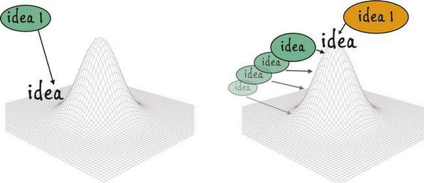
\includegraphics{img/Picture2.png}
    \end{subfigure}
    \begin{subfigure}
        \centering
        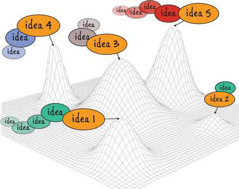
\includegraphics{img/Picture3.png}
    \end{subfigure}
\end{figure}

"Getting the Design Right" (links) vs. "Getting the Right Design" (rechts). Abbildungen aus \textcite{greenberg_2012}.

Stattdessen erst unterschiedliche Ideen mit sehr geringen Änderungskosten (= billige und grottige Papierskizzen) explorieren, dann erst für die beste Idee entschei-den (auf Basis der Nutzungsanforderungen, Ihren Fertigkeiten und zur Verfügung stehenden Zeit)!)

\begin{figure}[htbp]
    \centering
    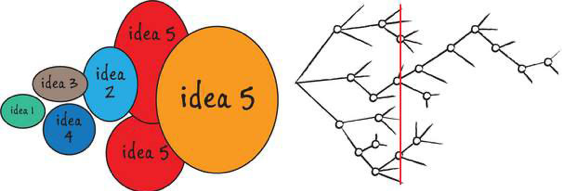
\includegraphics{img/Picture4.png}
\end{figure}

Abbildung aus \textcite{greenberg_2012}.

Die Konzeption \textbf{kann unterschiedlich aufgebaut sein} und \textbf{nicht alle Unterkapitel sind bei jeder Entwicklung relevant}. Die Struktur muss Sinn ergeben — im Zweifelsfall mit dem Betreuer abstimmen. Die Unterkapitel Konzeptionsvorgehen, Anwendungsfälle (Use-Cases) und Funktionalitäten wird man in den meisten Fällen benötigen. \textbf{Mögliche Reihenfolgen danach sind:}

\begin{itemize}
    \item \textbf{Iterationsweise:} Bietet sich an, wenn Sie nur einen Aspekt (z. B. nur das Interface) entwickeln. Sie beschreiben in eigenen Unterkapiteln die jeweiligen Iterationen samt formativer Evaluation, aus der sich dann die nächste Iteration ableitet.
    \item \textbf{Strukturell gegliedert:} Aufteilung in Unterkapitel (Systemarchitektur, Interface, etc.) und Beschreibung der Iterationen dieser in den jeweiligen Unterkapiteln.
\end{itemize}
\end{comment}

Text \dots

\section{Conceptual Approach}
\begin{comment}
Die Konzeption verläuft — noch stärker als die Analyse — iterativ. Die Unterkapitel sind allerdings linear strukturiert. Vergleichbar mit den Datenquellen der Analyse bietet sich das erste Unterkapitel an, das Vorgehen und die eingesetzten Methoden zu beschreiben (deren Ergebnisse sich meist in mehreren Unterkapitel niederschlagen).

\textbf{Methoden} können z. B. sein:

\begin{itemize}
    \item \textbf{Analyseworkshop:} Nützlich um die Ergebnisse der Analyse zu strukturieren und für die Konzeption aufzubereiten (vgl. \textcite[S. 190-192]{kumar_2013})
    \item \textbf{Design-Sprints:} Stärker für die Konzeption (vgl. \textcite{knapp_2016})
    \item \textbf{Workshops mit der Zielgruppe:} Generell um Ideen partizipativ zu entwickeln und formativ zu evaluieren.
\end{itemize}

Auch hier: Vorgehen beschreiben, Teilnehmer mit Alter (M, SD), Geschlecht (m/w/d) sowie relevanten Eigenschaften (warum stehen sie für die Zielgruppe?).

In den folgenden Unterkapitel können Sie dann auf 3.1 verweisen.
\end{comment}

Text \dots

\section{Use Cases}
\begin{comment}
Use Cases bieten sich an, die Ergebnisse aus der Analyse zusammenzufassen und in einen oder mehrere konkrete Anwendungsfälle zu übertragen. Die Tabelle mit den Nutzungsanforderungen sollte hierbei helfen. Wie sieht die Situation aus, wenn Ihr System eingesetzt wird? Bei den Anwendungsfällen noch nicht zu spezifisch werden. Es geht primär darum zu beschrieben, was die Person macht, z. B. veränderte Arbeitsabläufe, neue Funktionen, etc., noch nicht wie genau dies (technisch, womit realisiert) umgesetzt wird.
\end{comment}

Text \dots

\section{Functionalities}
\begin{comment}
Geben Sie einen Überblick über die geplanten Funktionalitäten des Systems. Dazu können Sie die Anwendungsfälle der Konzeption sowie die Tabelle mit den Nutzungsanforderungen aus der Analyse aufgreifen und den Anforderungen mögliche Funktionalitäten zuordnen. Priorisieren Sie dann diese Funktionalitäten — bezüglich Auswirkungen auf die Gebrauchstauglichkeit des Systems und Umsetzbarkeit dieser Funktionen.
\end{comment}

Text \dots

\section{System Architecture}
\begin{comment}
Mit den Funktionalitäten gehen bestimmte Anforderungen an das zugrundeliegende System einher. Stellen Sie hier dar, welche Lösungen es für die Systemarchitektur gibt, welche Aufteilungen sich eignen (z. B. MVC) und wie man es umsetzen könnte. Je nach Detailgrad bieten sich u.a. UML-Diagramme an.

\textbf{Begründete Auswahl:} Nehmen Sie die Funktionalitäten als Grundlage, das gibt Ihnen vor, mit welchen möglichen Architekturen Sie diese Funktionalitäten umsetzen können. Falls es mehrere Möglichkeiten gibt, erläutern Sie diese und treffen eine be-gründete Auswahl auf Basis dessen Stärken und Schwächen für Ihren Anwendungsfall.

\textbf{Hardware/Software-agnostisch bleiben:} Es geht hier explizit nicht um spezifische Hard- oder Software. Sie bleiben auf der "Datenbank", "Server", etc. Ebene. Welche Datenbank (MySQL, PostgreSQL, SQLite, etc.) oder welcher Server (Apache, Node.js, etc.) verwendet wird kommt in der Realisierung. Auch hier: Nach der Konzeption kann der Leser stoppen und Ihre Konzeption auf seine Weise realisieren.

\textbf{Bezug zum Interface Design beachten:} Systemarchitektur und Interface Design hängen eng zusammen. Stimmen Sie beides aufeinander ab — in jeder Iteration.
\end{comment}

Text \dots

\section{Interface Design}
\begin{comment}
Wie können die Informationen dargeboten und Angaben der Nutzer erfolgen?

\textbf{Screen-Fetisch hinterfragen:} Viele Medieninformatiker haben einen Fetisch was visuelle Interface betrifft. Diese lassen sich leicht skizzieren, es gibt Tools dafür, die man kennt, und man kann was zeigen. Man sieht, was man gemacht hat. Für viele Kontexte sind sie allerdings absolut ungeeignet (z. B. um Autofahrer zu energiesparendem Fahren zu bringen). Visuelle Aufmerksamkeit ist extrem kostbar. Probieren Sie deswegen bewusst andere Sinne aus. Können Sie die Informationen auch auditiv geben (z. B. Abweichung vom idealen Fahrverhalten über die Tonhöhe)? Oder haptisch (z. B. Vibration)? Gerade wenn man sich im Laufe der Konzeption in das eigene visuelle Design verliebt kommen oft Lösungen heraus, die vielleicht schön sind, aber auch lebensgefährlich, und schlimmer noch: nicht gebrauchstauglich. Für viele Kontexte sind visuelle Interfaces sehr gut geeignet — aber für viele auch nicht. Und die Auswahl sollte wie üblich begründet erfolgen.

\textbf{Formativ Evaluieren:} Interface-Designs müssen Sie formativ evaluieren. Für Sie ist die Interaktion klar (Sie wissen auch als — meist — einzige Person, was unter der Oberfläche passiert und was die Hintergründe sind), für Laien ist das oft unklar. Sie brauchen früh Feedback der Zielgruppe. Nutzen Sie es! Dokumentieren Sie am Ende jeder Iteration, was herausgekommen ist und was die Konsequenzen für Ihr Design / die nächste Iteration war.

\textbf{Papier über Mock-Up-Tools:} Verwenden Sie Papier um visuelle Interfaces zu gestalten. Wenn Sie nicht zeichnen können, um so besser. Bei mit dem Computer ausgearbeiteten Mockups ist die Hemmung der Zielgruppe oft zu hoch, noch grundlegende Aspekte zu ändern. Damit bleiben Sie oft in der ersten — und oft unkreativen und nicht gebrauchstauglichen — Lösung gefangen. Tools wie Adobe XD sind eine Falle, die Sie zumindest in den ersten Iterationsphasen tunlichst vermeiden sollten.

\textbf{Bei visuellen Interfaces Skizzen der Iterationen darstellen:} Benutzen Sie Graphiken (Skizzen, Mockups) um das Interface und die Interaktion damit zu verdeutlichen.
\end{comment}

Text \dots

\newpage
\begin{comment}
\begin{center}
\huge
Nach der ersten Iteration:\\STOP\\
\normalsize
Nachdem Sie die erste Iteration abgeschlossen haben, nehmen Sie das Blatt Papier, auf dem Sie vor/während der Analyse Ihre Lösungsidee(n) festgehalten haben, wieder heraus. Vergleichen Sie Ihre ursprüngliche Idee mit der ersten Iteration.

\textbf{Falls sich Ihre erste Iteration sich stark von der erste Idee unterscheidet:} Prima. Sie haben während der Analyse dazu gelernt und den Nutzungskontext besser verstanden. Ohne die Analyse und die Verwendung dieser Informationen in der Konzeption hätten Sie das nicht machen können.

\textbf{Falls Ihre erste Iteration Ihrer ersten Idee sehr ähnlich ist:} Entweder Sie kannten sich schon vor der Analyse mit dem Themengebiet sehr gut aus — oder (und das ist wahrscheinlicher) — sie hängen zu stark an Ihrer ersten Idee und hören der Zielgruppe nicht zu. Auch falls Sie selbst zur Zielgruppe gehören (z. B. eine Anwendung für Studierende), Sie sind nicht "alle Nutzer". Nutzer unterscheiden sich üblicherweise. Entsprechend wirklich am in sich gehen — haben Sie aus der Analyse wirklich nichts dazu gelernt? Was das Problem (oder Sie selbst) wirklich so trivial? Das Schöne an kreativen Prozessen ist ja, dass man iterativ besser werden kann und auch auf Ideen kommen kann, auf die man vorher nicht gekommen wäre. Die Chance sollten Sie nutzen.

BTW, dieser Hinweis heißt nicht, dass Sie komplett naiv an Ihre Gestaltung herangehen sollten, ohne sich vorher Gedanken zu machen. Aber, wenn Sie eine Analyse wirklich ernst nehmen, dann sollte die Ihnen Sachverhalte aufzeigen, die man als Außen-stehender nicht sieht. Und Sie sollten auch in der Konzeption basierend auf diesen Informationen Lösungen entwickeln, die über die ersten simplen Ideen hinausgehen (vgl. confirmation bias). Die neu und nützlich sind.
\end{center}
\end{comment}

\section{Conclusion on the Conception}
\begin{comment}
Wie auch bei der Analyse am Ende der Konzeption ein kurzes Fazit um den Entwicklungsprozess zusammenzufassen und begründen, was die erfolgversprechendste Lösung (höchste Gebrauchstauglichkeit in der formativen Evaluation!) für die Realisierung ist.
\end{comment}

Text \dots

\newpage
\chapter{Implementation}
\begin{comment}
Beschreiben Sie, wie Sie das Projekt konkret realisiert haben, mit dem Ziel, anderen (Medien-)Informatikern zu erlauben, Ihre Anwendung weiter zu entwickeln.

\textbf{Test:} Sie nehmen einen Kommilitonen, geben ihm dieses Kapitel und bitten ihm eine Funktion hinzuzufügen oder zu verändern. Wenn er das kann, prima. Wenn nicht, besser schreiben oder bessere Kommilitonen suchen.

Verweisen Sie zu Beginn auf die erfolgreichste Lösung aus der Konzeption. Wie in der Konzeption bieten sich Unterkapitel mit Systemarchitektur und Interface-Design an — jetzt allerdings mit konkreten Angaben, welche Programme / Frameworks Sie verwenden, und wie Sie das Interface konkret umsetzen.

Geben Sie zuerst einen allgemeinen Überblick und werden dann konkreter. Als wenn Sie in eine Weltkarte reinzoomen. Erst mal sagen, wie die Welt aufgebaut ist (Kontinente), dann auf Kontinent mit Ländern zoomen, dann exemplarisch mal auf ein Land. Leser braucht ein gutes mentales Modell vom Aufbau und den Funktionen, um zu verstehen, wie es technisch umgesetzt wurde.

\textbf{Begründen Sie Ihre Entscheidungen linear:} Z.B.

\begin{enumerate}
    \item "das sind die Anforderungen aus der Analyse/bisheriger Konzeption"
    \item "Programmiersprache / System / etc. x, y, und z erfüllen diese Anforderungen"
    \item "relevante Kriterien sind a, b, c und d (z. B. Verbreitung, Community, Weiterentwicklung, Preis)"
    \item "Programmiersprache / System / etc. x, y, und z schneiden da so und so ab, x ist insgesamt am besten"
    \item "Programmiersprache / System / SDK / etc. x wird verwendet". Eine Argumentation à la A => B => C => D => E ist nachvollziehbarer als wir nehmen E, weil A => C woraus D folgt, wegen B.
\end{enumerate}

Weiterer Grund: Wenn Sie zuerst die konkrete Software sagen, dann fangen Personen direkt an, die Entscheidung zu hinterfragen (weil sie z. B. eine andere bevorzugen, gibt da genug Religionskriege). Wenn Sie linear argumentieren gehen diese Personen eher bei jedem Schritt mit und enden dann bei der von Ihnen verwendeten Software (sofern sie bei den Auswahlkriterien und der Bewertung mitgehen).

\textbf{Nutzen Sie den Datenträger im Anhang der Arbeit:} Insbesondere in den Programmcode können Sie viel auslagern. In der Arbeit muss der Leser aber die Struktur/den Aufbau Ihres Programms verstehen sowie die Logik dahinter. Und er muss wissen, dass es die Erläuterungen im Programmcode gibt und wo er diese findet. Entsprechend die Struktur (Dateien/Klassen) deutlichen machen und Verweise auf relevanten Dateien.
\end{comment}

Text \dots

\section{System Architecture Implementation}
\begin{comment}
vgl. Konzeption, jetzt aber wie und womit es konkret umgesetzt wurde (u.U. bieten sich UML-Diagramme an)
\end{comment}

Text \dots

\section{Interface Implementation}
\begin{comment}
vgl. Konzeption, jetzt aber wie und womit es konkret umgesetzt wurde 
\end{comment}

Text \dots

\section{Conclusion on the Implementation}
\begin{comment}
Kurzes Fazit, das u.a. die Frage beantwortet, was technisch konkret umgesetzt wurde und was z. B. aus der Konzeption übrig geblieben ist und warum.
\end{comment}

Text \dots

\newpage
\chapter{Dialogue Samples}
\begin{comment}
Verdeutlichen Sie die Funktionsweise Ihre Entwicklung bei einer typischen Bedienung (z. B. wie in einem Anwendungsbeispiel / Use Case beschrieben — auf den können Sie sich ja beziehen).

Die Abbildungen müssen im Text vorher erläutert sein und einen Eindruck geben, wie die Entwicklung konkret bedient wird bzw. was sie kann.

\textbf{Das ist das, was bleibt:} Diese Dialogbeispiele sind das einzige, was in ein paar Jahren von Ihrer Anwendung noch sichtbar ist. Dann ist entweder der Datenträger verschwunden oder beschädigt oder die notwendige Hard- und Software ist nicht mehr lauffähig. Geben Sie dem Leser entsprechend einen guten Einblick in das, was Sie tatsächlich realisiert haben.

\textbf{Jetzt ein Video aufnehmen:} Schalten Sie den Screenrecorder auf dem Computer (not-falls: QuickTime) oder Smartphone (kann das OS) an und nehmen Sie die typischen Interaktionen einmal auf. Das ist Ihr "Plan B", falls (oft: wenn) im Kolloquium die App nicht bedient werden kann. Das können Sie auch gut auf DVD brennen um Lesern die Möglichkeit geben, sich die Interaktion anzusehen (in der Arbeit darauf hinweisen!). Macht sich auch gut auf Websites (insbesondere dem eigenen Portfolio).
\end{comment}

Text \dots

\newpage
\chapter{Summative Evaluation}
\begin{comment}
Geben Sie zu Beginn der Evaluation einen kurzen Überblick über Ihr Vorgehen. Dazu reichen meist die Zwischenüberschriften mit ein oder zwei Sätzen, was Sie konkret gemacht haben. Also nicht "In Design wird das Design beschrieben" sondern "Das experimentelle Vorgehen wird im Abschnitt Design dargestellt".
\end{comment}

Text \dots

\section{Goal}
\begin{comment}
Die summative Evaluation ist eine abschließende Bewertung Ihrer Entwicklung. Ziel ist, unter dem Strich zu sehen, wie gebrauchstauglich Ihr System ist (nicht mehr eine iterative Verbesserung wie in der formativen Evaluation der Konzeption). Da-für müssen Sie klare Kriterien ableiten, was eine "gute" bzw. "schlechte" Bewertung nach sich ziehen würde. Meist sind das die klassischen Gebrauchstauglichkeitskriterien (Effektivität, Effizienz, Erlernbarkeit, Zufriedenstellung), wobei diese über das Ziel Ihrer Anwendung konkretisiert werden (Effektivität bei einer Lernapp ist konkret gemessen etwas anderes als Effektivität bei einem digitalen Depressionstagebuch).

Hier verdeutlichen Sie entsprechend, welche Fragen die Evaluation beantworten soll.
\end{comment}

Text \dots

\section{Methods}
\begin{comment}
Im Methodenteil zeigen Sie, was wie evaluiert wurde. Der Methodenteil muss anderen Entwicklern die Möglichkeit geben, Ihr Evaluationsvorgehen zu wiederholen um Ihre Ergebnisse zu überprüfen. 
\end{comment}

Text \dots

\subsection{Design}
\begin{comment}
Kurze Beschreibung des Versuchs- oder Evaluationsdesigns, dass man das Vorgehen einordnen kann. Also z. B. "es wurde ein Usability Test durchgeführt", oder "es wurde ein Experiment mit between-subjects design durchgeführt, bei dem die Kontrollgruppe die bisherige App verwendet hat und die Experimentalgruppe die neu entwickelte App".
\end{comment}

Text \dots

\subsection{Participants}
\begin{comment}
Kurze Beschreibung der Teilnehmer mit relevanten Angaben. In jedem Fall die Anzahl, oft noch Geschlecht, Alter, Beruf, Vorerfahrung, etc. Bei weniger als zehn Teilnehmern bietet sich eine Tabelle zur schnellen Übersicht an. Verweisen Sie bei individuellen Ergebnissen (z.B. Zitaten aus Fragebögen oder Interviews) auf die Teilnehmer-Nummer.

Achtung: Niemals die Namen der Teilnehmer erwähnen! Die Teilnehmer stehen stellvertretend für die Zielgruppe. Wer sie konkret sind ist irrelevant. Begründen Sie, warum Sie diese Personen ausgewählt haben (spiegeln die Nutzergruppe gut wider) und wo/wie Sie diese rekrutiert haben.
\end{comment}

Text \dots

\subsection{Setting and Instruments}
\begin{comment}
Beschreiben Sie die notwendigen Materialien bei der Evaluation. Dazu gehört — mit Überschriften klar ausgewiesen — das Setting (wo wurde die Evaluation durchgeführt), Ihre Entwicklung (Verweis auf Dialogbeispiele), und Ihre Erhebungsmethoden (Fragebögen, Interviewleitfäden, etc.).

Falls Sie etablierte Fragebögen verwenden (z.B. ATI) reicht die entsprechende Zitation mit einer kurzen Beschreibung. Bei längeren Fragebögen oder Interviewleitfäden nennen Sie kurz die Abschnitte (z.B. soziodemographische Daten, Technikerfahrung, etc.) und verweisen Sie auf die vollständigen Fragebögen im Anhang.

\textbf{ACHTUNG:} Zeitliche Reihenfolge ist hier egal. Hier geht es nach Gliederungspunkten wie Instrumente (Fragebögen, Interviews, etc.). Die zeitliche Reihenfolge wird in der Prozedur dargestellt.
\end{comment}

\paragraph{Setting}\mbox{} \\
Text \dots

\paragraph{Verwendete Anwendung}\mbox{} \\
Text \dots

\paragraph{Fragebögen}\mbox{} \\
Text \dots

\subsection{Procedure}
\begin{comment}
Beschreiben Sie chronologisch den Ablauf der Evaluation, von der Begrüßung bis zur Verabschiedung. Verweisen Sie dabei auf die anderen Abschnitte (v.a. Setting und Instrumente) und führen Sie nichts Neues mehr ein. Dieser Abschnitt ist der einzige Abschnitt, in dem Sie die zeitliche Reihenfolge klar einhalten müssen, alle anderen sind inhaltlich strukturiert.
\end{comment}

Text \dots

\begin{comment}
Nach dem Lesen der Methode muss deutlich geworden sein, wie Sie Ihre Evaluationsfragen messbar gemacht haben. Wie haben Sie z.B. Benutzerzufriedenheit oder Effizienz gemessen? Die Leser müssen sich aufgrund des Methodenteils in die Lage der Teilnehmer versetzen können und ein mentales Modell Ihrer Evaluation bilden können.
\end{comment}

\section{Results}
\begin{comment}
In den Ergebnissen zeigen Sie wie die Ergebnisse analysiert wurden um Ihre Evaluationsfragen zu beantworten. Nicht einfach die Daten auflisten, sondern stellen Sie die Ergebnisse strukturiert dar und betonen Sie die wichtigen Aspekte. Gliedern Sie die Ergebnisse nach Ihren Forschungsfragen / Fragestellungen (nicht zeitlich oder nach Erhebungsmethoden wie Fragebögen vs. Beobachtung). Zu Beginn (falls relevant) sollten Sie überprüfen, ob die Anwendung auch wirklich so verwendet wurde, wie sie verwendet werden sollte (manipulation check). Haben die Personen also z. B. wirklich die Aufgaben mit der App gelöst oder haben sie die App schnell beiseite gelegt.

Stellen Sie die Befunde / Ergebnisse von Analysen / Evaluationen / etc. immer so neutral und so objektiv wie möglich dar — ohne Ihre subjektive Interpretation oder Bewertung. Also keine Begriffe wie "lediglich", "nur", "könnte / würde / sollte / etc." oder Bewertungen wie "hat gut / nicht gut geklappt". Diese Bewertungen gehört in die Diskussion.

Überlegen Sie sich mit welchen Tabellen und Abbildungen Sie die Ergebnisse gut darstellen können. Bei aggregierten Messwerten (auf mindestens Intervallskalenniveau) immer Mittelwerte (M), Standardabweichungen (SD) und die Anzahl der Messdaten (Personen, n) angeben. Bei ordinalskalierten Daten entsprechend Median, etc. (ja, Statistik war wichtig).

Statistische Tests korrekt angeben (siehe z.B. Pallant, 2010).

Pallant, J. (2007). SPSS Survival Manual (3rd ed.). Open University Press.

Abbildungen müssen in sich verständlich sein (was abgebildet ist). Das heißt, die Achsen eindeutig beschriften, Skala (z.B. Likert-Skala von 1 starke Ablehnung bis 7 starke Zustimmung) in die Legende. 3D-Graphiken vermeiden — diese bieten oft keinen Mehrwert (vgl. Field, 2016).

Field, A. (2016). An Adventure in Statistics. Sage.

Am Ende des Ergebnis-Abschnitts muss deutlich geworden sein, wie Ihre Entwicklung von den Teilnehmenden eingesetzt wurde (hoffentlich wie geplant), was die Hauptergebnisse waren, sofern aufgrund der Stichprobengröße möglich welche Werte sich statistisch signifikant voneinander unterscheiden und was die statistischen Ergebnisse in den Variablen bedeuten (z. B. positive Korrelation zwischen A und B, dass Personen, die A besser bewertet haben auch B besser bewertet haben; aber keine Bewertung ob das gut oder schlecht ist). Falls Sie konkrete Ziele hatten (z. B. "SUS-Wert von x") dann sagen Sie, ob dieses Ziel erreicht wurde oder nicht (das ist keine Wertung, die in die Diskussion gehören würde, sondern ein größer, gleich oder kleiner was eindeutig ist).
\end{comment}

Text \dots

\section{Discussion}
\begin{comment}
In der Diskussion erklären und interpretieren Sie die Ergebnisse. Welche Schlussfolgerungen ziehen Sie daraus? Was sind die praktischen Konsequenzen für die (weitere) Entwicklung? Hier dürfen Sie selbst die Ergebnisse bewerten — auf Basis von einer kritischen Reflektion.
In der Diskussion keine neuen Ergebnisse aus der Analyse / Evaluation / etc. einführen. Die Beweisaufnahme ist mit Ende des Ergebnisteils abgeschlossen. Es geht hier auch nicht um eine Mystery-Geschichte mit Spannungsbogen, sondern um klar nachvollziehbare Argumente. Neue Informationen aus der Literatur verwenden um die (v.a. überraschende) Ergebnisse zu interpretieren ist dagegen möglich.
\end{comment}

Text \dots

\section{Conclusion on the Evaluation}
\begin{comment}
Fassen Sie die Evaluation kurz zusammen — insbesondere was die zentralen Ergebnisse waren. Unterm Strich: Wie gut hat's geklappt?
\end{comment}

Text \dots

\newpage
\chapter{Summary and Outlook}
\begin{comment}
Kurze Einführung, was in den folgenden Unterkapiteln behandelt wird.
\end{comment}

Text \dots

\section{Summary}
\begin{comment}
Fassen Sie die zentralen Schritte und Ergebnisse Ihrer Arbeit kurz zusammen. Personen mit wenig Zeit müssen aus dieser Darstellung die Kernpunkte Ihrer Arbeit mit-nehmen und Ihren Arbeitsaufwand und Erfolg bewerten können.

Ist ähnlich wie die Zusammenfassung zu Beginn der Arbeit, aber etwas länger (1 bis maximal 2 Seiten) mit Verweisen auf die entsprechenden Kapitel/Abschnitte und Sie können beim Leser etwas mehr voraussetzen (hat es gelesen oder kann wegen den Verweisen direkt dahin springen).
\end{comment}

Text \dots

\section{Outstanding Issues}
\begin{comment}
\textbf{Offene Punkte = Versprochene aber nicht umgesetzte Punkte:} Falls Schritte explizit geplant wurden (Exposé! Pflichtenheft!), aber nicht realisiert werden konnten, dann diese hier klar darstellen und diskutieren.

Mögliche Features, die Sie nicht vor Beginn versprochen haben, gehören in den Ausblick.
\end{comment}

Text \dots

\section{Outlook}
\begin{comment}
Ideen, welche weiteren Entwicklungen oder Untersuchungen folgen sollten, oder was man noch umsetzen könnte, gehören in den Ausblick.

Versprochene aber nicht umgesetzte Elemente in die Offenen Punkte.

Bitte keine Allgemeinheiten ("können noch Features hinzugefügt werden" oder "könnte besser evaluiert werden") sondern konkrete Beschreibungen und Begründungen der Relevanz dieser Schritte.
\end{comment}

Text \dots

\section{Final Conclusion}
\begin{comment}
Die Arbeit, die Ergebnisse und weitere mögliche Schritte kurz kritisch (ehrlich und konstruktiv, aber nicht selbstkreuzigend) reflektieren und positiv enden. Maximal eine halbe bis 3/4 Seite.
Ist kurz und hier können Sie von der Arbeit zurücktreten und auch den Leser aus dem Text ziehen.

Das ist nur zum Test: \textcite{ford} \textcite{hadoop}
\end{comment}

Text \dots

\clearpage
\phantomsection
\addcontentsline{toc}{chapter}{Abbildungsverzeichnis}
\listoffigures
\clearpage

\phantomsection
\addcontentsline{toc}{chapter}{Tabellenverzeichnis}
\listoftables
\clearpage

\phantomsection
\addcontentsline{toc}{chapter}{Quellen}
\chapter*{Quellen}

\phantomsection
\printbibliography[heading=subbibintoc, nottype=online, nottype=software]

\phantomsection
\printbibliography[heading=subbibintoc, type=online, title=Websites]
\begin{comment}
Websites haben nicht die gleiche Fundierung/Überzeugungskraft wie wissenschaftliche Literatur (peer-review/Anspruch). Die Websites separat aufzuführen, macht es einfacher zu sehen, was wirklich wissenschaftlich fundierte Literatur ist.
\end{comment}

\phantomsection
\printbibliography[heading=subbibintoc, type=software, title=Software]
\begin{comment}
Software-Name mit Versionsnummer und Link zur Website. Nur was für die konkrete Arbeit relevant ist. Das Sie die Arbeit mit Word geschrieben haben, ist irrelevant. Das sieht man. LaTeX auch.
\end{comment}
\clearpage

\phantomsection
\addcontentsline{toc}{chapter}{Abkürzungen}
\chapter*{Abkürzungen}
\begin{comment}
Kann recht kurz ausfallen, aber falls Sie bestimmte Abkürzungen häufiger verwenden, hier aufführen. Geht nur darum, dass der Leser hierhin blättern könnte, wenn er über eine unbekannte Abkürzung stolpert. Ist beim digitalen Lesen hinfällig geworden. Hier geht es wirklich nur um Akronyme, z. B. ICBM = Intercontinental Ballistic Missile, oder PIN = Personal Identification Number. Die Erläuterung von Begriffen erfolgt im Glossar.
\end{comment}

\begin{description}
    \item [\textbf{Akronym}] Ausgeschriebenes Akronym
\end{description}
\clearpage

\phantomsection
\addcontentsline{toc}{chapter}{Glossar}
\chapter*{Glossar}
\begin{comment}
Unterschiedliche Disziplinen verwenden z. T. die selben Begriffe für unterschiedliche Sachverhalte und unterschiedliche Begriffe für die selben Sachverhalte. Hier können Sie wiederkehrende zentrale Begriffe der Arbeit kurz definieren (z. B. Adipositas, Depression, Legasthenie, etc.). Früher wichtiger, dann konnte man hierhin blättern und musste nicht den ganzen Text absuchen. Heute verwendet man digital die Suchfunktion. Trotzdem ernst nehmen.
\end{comment}

\begin{description}
    \item [\textbf{Begriff}] Kurze Erläuterung
\end{description}
\clearpage

\phantomsection
\addcontentsline{toc}{chapter}{Anhänge}
\chapter*{Anhänge}
\begin{comment}
Zusätzliche Informationen die zu lang für die Arbeit sind können hier verfügbar gemacht werden.

Aber auch an die DVD denken — was ist dort besser aufgehoben? Die Zeiten, in denen man Programmcode manuell eingetippt hat, sind ja glücklicherweise lange vorbei, deswegen macht Code hier wenig Sinn.

Ist entsprechend ein Priorisierung: Was würde sich der Leser vielleicht gerne während des Lesens der Arbeit (z. B. im Zug) ansehen, wenn er auch gerade nicht auf die DVD zugreifen kann (kein DVD Laufwerk)?

Inhalte sind oft: Überblick der Inhalte der DVD, Fragebögen (falls digital Screenshots oder neu für den Druck formatiert), Interviewleitfäden, etc. Selten detailliertere Evaluationsergebnisse.

Hier kurz die Zwischenüberschriften nennen und evtl. 1 Satz, was dort zu finden ist (falls es nicht schon durch die Zwischenüberschrift klar ist). 
\end{comment}

Text \dots

\phantomsection
\addcontentsline{toc}{section}{Anhang A: Inhalt der DVD}
\section*{Anhang A: Inhalt der DVD}
\begin{comment}
Oft ein Default: Was findet man auf der beiliegenden DVD in welchem Verzeichnis? Max. 1 Seite.

\textbf{In jedem Fall} die PDF der Arbeit, den Programmcode, Daten (anonymisiert!).

\textbf{Niemals} Interviewaufzeichnungen, Einverständniserklärungen oder ähnliche personenbezogene Daten auf die DVD brennen — Sie haben in den meisten Fällen Anonymität zugesichert und die DVD ist frei zugänglich (ein Exemplar der Arbeit kommt in die Bibliothek). 
\end{comment}

Text \dots

\phantomsection
\addcontentsline{toc}{section}{Anhang B: Anhangstitel}
\section*{Anhang B: Anhangstitel}
\begin{comment}
Weitere Inhalte je nachdem, wo der Leser ohne großen Aufwand hinspringen sollte.
\end{comment}

Text \dots

\clearpage

\phantomsection
\addcontentsline{toc}{chapter}{Erklärung}
\chapter*{Erklärung}
Ich versichere an Eides statt, die vorliegende Arbeit selbstständig verfasst und nur die angegebenen Quellen benutzt zu haben.

\begin{comment}
[Nach Ausdruck unterschreiben. Muss auf Papier sein.]
\end{comment}

-----------------------------------------------------------------

Lübeck, \today, \authorMA
\end{document}
